\section{Color Transparency at High Energies}
\label{sec:ct_high_energies}

For $l_c$ greater than the nuclear radius, one can treat a PLC as a
``frozen'' $q\bar{q}$ dipole with transverse size
$d$~\cite{Blattel_1993, Frankfurt_1993}.
Then in the leading log approximation, the dipole-nucleon cross section is
given by~\cite{Frankfurt_2000, Frankfurt_2002}
\begin{equation} \label{eq:dipole_cross_section}
    \sigma_{q\bar{q} N}^{inel}(d,x) = \frac{\pi^{2}}{3} \alpha_{s}
    \left( Q_{eff}^2 \right) d^2
    \left[
           x G_{N} \left( x, Q_{eff}^2 \right) +
           \frac{2}{3} x S_{N} \left( x, Q_{eff}^2 \right)
    \right].
\end{equation}


Here $Q_{eff}^2=\lambda/d^2$, $x=Q_{eff}^2/s$, $s$ is the invariant energy of
the dipole-nucleon system, and $S$ and $G$ are the sea quark and gluon
distributions making up the dipole.
The parameter $\lambda$ takes a values between 4 and 10, and was estimated by
matching this model with the leading log description of
$\sigma_L(x,Q^2)$~\cite{Frankfurt_1996}.


\subsection{$J/\psi$ photoproduction}
% TODO: Link $J/\psi$ historically to CT.
% The $J/\psi$ decay width is narrow and photoproduction cross section is small.
% In 1974, argument given for why a heavy quark system should have a radius
% smaller than ``the one given by pion emission.'' %?
% ABOVE: L. L. Frankfurt and V. A. Khoze, in Proceedings of 10th LNPI Winter
% School, Leningrad, USSR, 1975, v2,pp 196-408; Yad.Fiz. 23 926 (1976).
%
% Fermi had previously argued that hadrons' radii were determined by the pion
% clooud and should all thus be approximately the same. % citation?
% https://arxiv.org/pdf/0711.1625.pdf has an expanded version of this claim

The $A$-dependence of $J/\psi$ production by real photons was studied at
Fermilab, providing the first experimental evidence of CT~\cite{Sokoloff_1986}.
A beam of \SI{210}{\giga\electronvolt} electrons passed through 0.53 radiation
lengths of material, generating \SIrange{80}{190}{\giga\electronvolt} bremsstrahlung
photons.
These real photons passed through both a \SI{1}{\m} \ch{LH2} target and one of
three solid targets (Be, Fe, and Pb) which were alternated throughout the run
period.
A lead absorber shielded detectors from electromagnetic showers generated in
the targets.
Relative per-nucleon cross sections were computed from dimuon $p_T^2$ spectra
measured for each target in the Tagged Photon Spectrometer.


The photoproduction process proceeds in three stages~\cite{Brodsky_1994};
the photon converts to a small $c\bar{c}$ pair before it gets to the target,
passes through the target with little expansion,
and converts to $J/\psi$ outside the target.


The measured cross section can be fit to a power law, $\sigma_{coh} =
\sigma_0 A^\alpha$.
A vector-meson-dominance model~\cite{Bauer_1978} of coherent photoproduction
predicts the per-nucleon cross section grows like $A^{4/3}$ at high energies,
provided interactions between $J/\psi$ and nucleons are small.
Using more realistic nuclear wavefunctions predicts $A^{1.40}$.
Consistent with this prediction, the experiment measured
$\alpha_{coh} = 1.40 \pm 0.06 \pm 0.04$, which can be interpreted as a result
of CT.
% incoherent Jpsi prediction makes less sense to me. TODO: revisit.


\subsection{Pion dissociation into two jets}
Consider a high momentum pion undergoing a coherent interaction with a nucleus
The final state consists of two jets with high transverse relative momentum
$k_T$ and the nucleus still in its ground state.
This $q\bar{q}$ Fock component of the pion should dominate this process.
Since momentum transfer to the nucleus is very small, the large transverse
momentum $k_T$ must originate in gluonic interactions between the quark and
antiquark.
In addition, this large $k_T$ means the $q\bar{q}$ pair must be in a PLC.
Indeed, a model-independent analysis of the pion form factor~\cite{Miller_2011}
showed that the pion's transverse charge density is sharply peaked at small
distances, consistent with a PLC, as shown in
Figure~\ref{fig:pion_charge_density}.


The amplitude for this process, given the cross section in
equation~\ref{eq:dipole_cross_section}, is
\begin{equation}
    A(\pi N \rightarrow 2 j e t s+N)\left(z, p_{t}, t=0\right) \propto
    \int d^{2} d \psi_{\pi}^{q\bar{q}}(z,d) \sigma_{q\bar{q}-N(A)}(d,s) e^{i p_t d}
\end{equation}


The normalization is determined by the Brodsky-Lepage relation~\cite{Lepage_1980}:
\begin{equation}
    \psi_\pi^{q\bar{q}}{\left(z,d\right)}_{d\rightarrow0} = \sqrt{48} f_\pi z (1-z)
\end{equation}


\begin{figure}[!h]
    \centering
    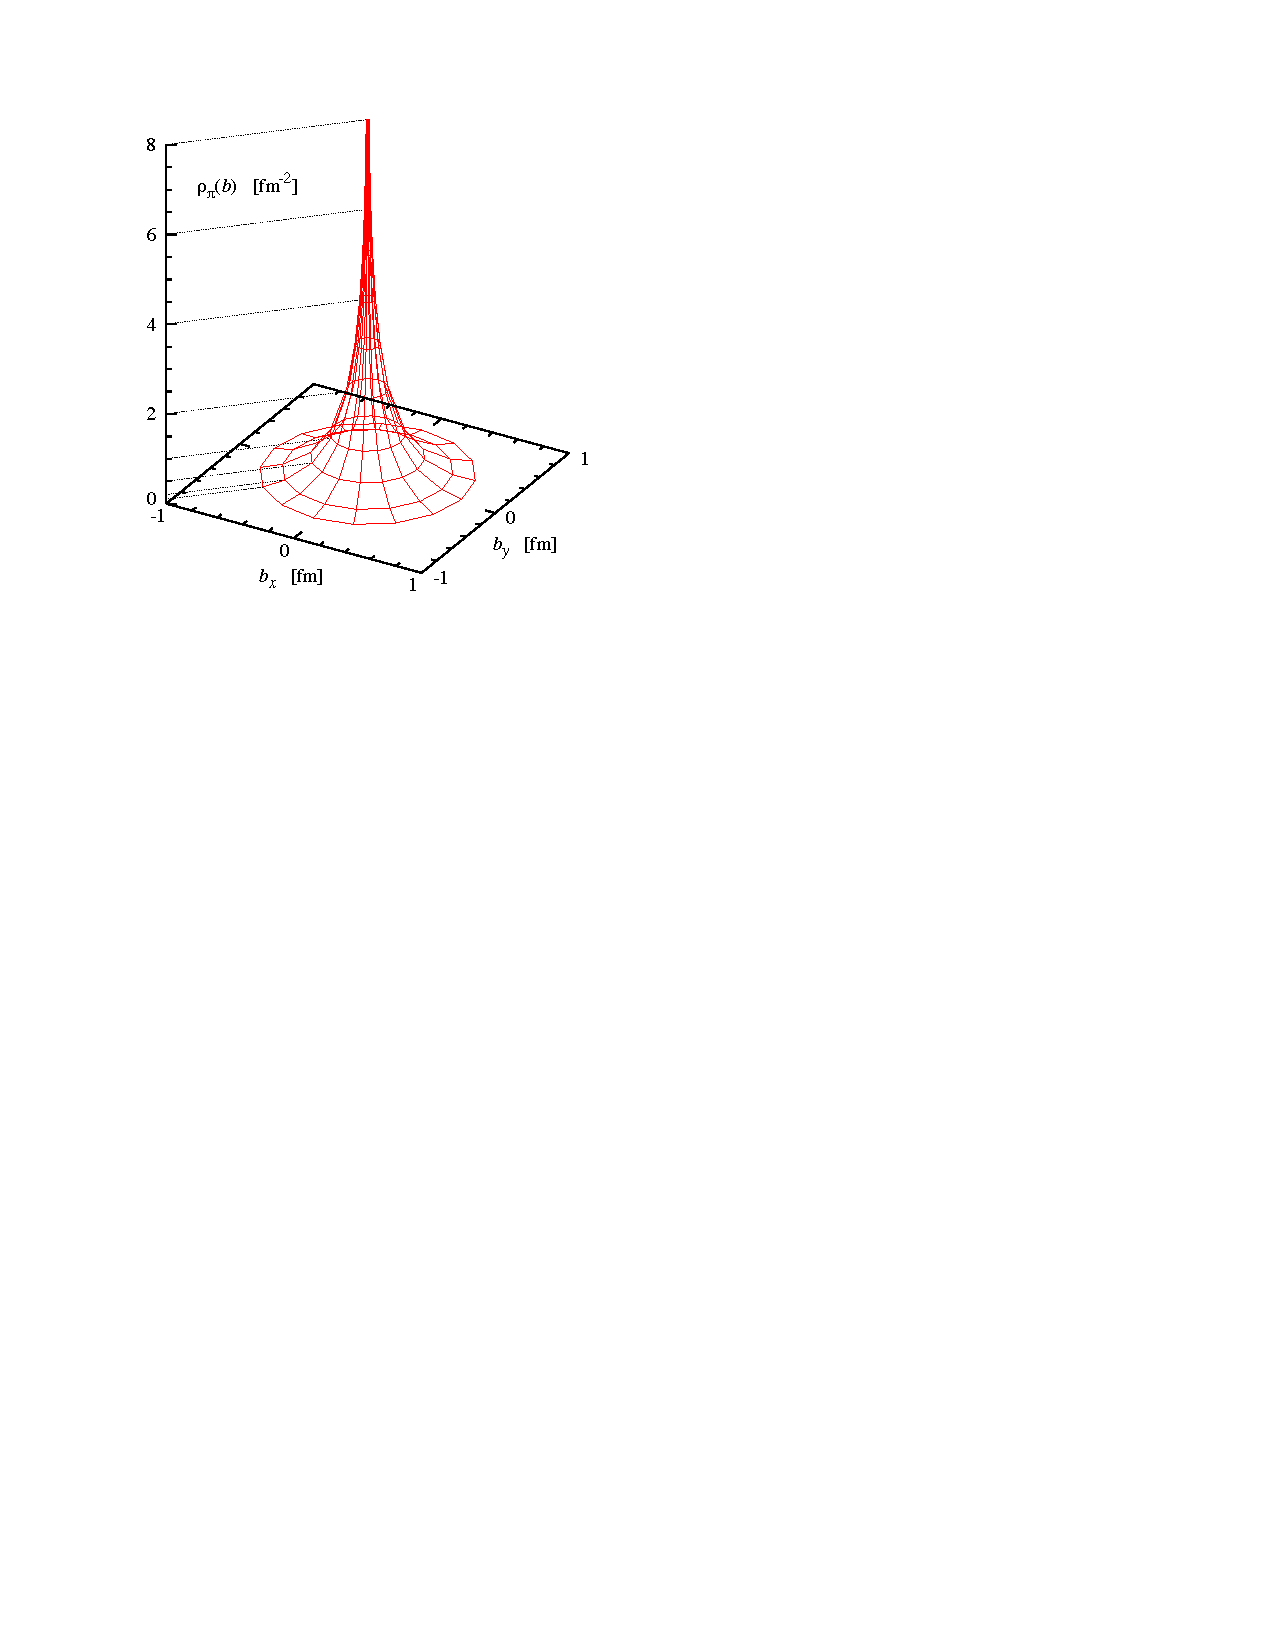
\includegraphics[width=0.6\textwidth]{chap2/pion_charge_density.pdf}
    \caption{Three-dimensional rendering of the pion's trasnverse density, as
             calculated in Ref~\cite{Miller_2011}.
            }
    \label{fig:pion_charge_density}
\end{figure}


The E791 experiment at Fermilab studied diffractive dissociation into dijets of
\SI{500}{\giga\electronvolt} pions~\cite{Aitala_2001_1, Aitala_2001_2}
scattering coherently from carbon and platinum targets.
As with $J/\psi$ photoproduction, the per-nucleon cross section can be fit to
$\sigma = A^\alpha\sigma_a$.
Frankfurt et al.~\cite{Frankfurt_1993} predicted that this cross section's
$A$-dependence should depend on $k_T$, the transverse momentum of each jet with
respect to the beam axis.
The E791 experiment calculated $\alpha$ for three different $k_T$ bins
Their results are shown in Figure~\ref{fig:pion_dijet_alpha} along with the
predictions of~\cite{Frankfurt_1993}.

\begin{figure}[!h]
    \centering
    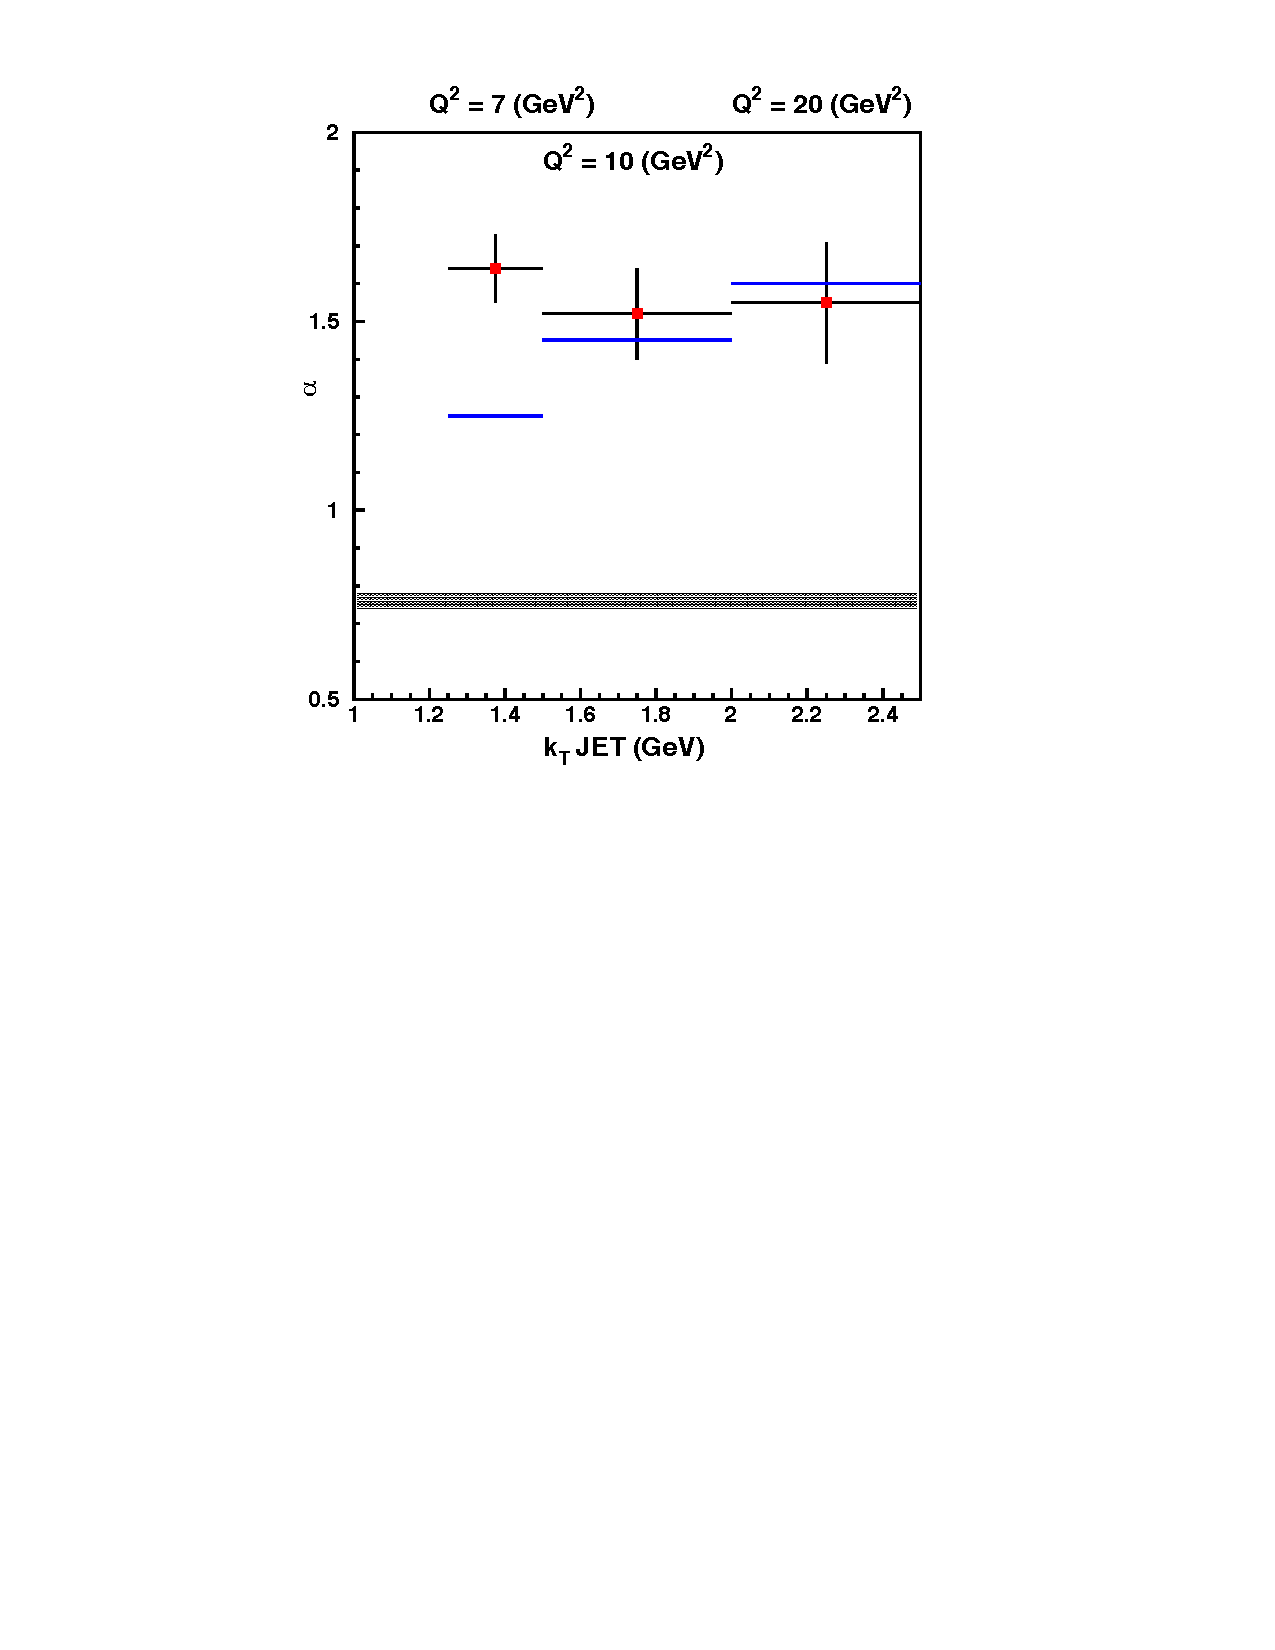
\includegraphics[width=0.6\textwidth]{chap2/pion_dijet_alpha.pdf}
    \caption{The results of a parameterization, $\sigma=A^\alpha\sigma_0$, of
             the cross section for pion dissociation into two jets.
             The values from data are shown as red points with statistical and
             systematic errors added in quadrature.
             The lines represent the CT-based predictions
             of~\cite{Frankfurt_1993}.
             The shaded band represents the value $\alpha\sim2/3$ typical of
             coherent inelastic diffractive pion-nucleus
             interactions~\cite{Zielinsk_1983}.
            }
    \label{fig:pion_dijet_alpha}
\end{figure}


% TODO:
Summarize why this is a good result.

\subsection{Vector meson production}
The leading twist picture~\cite{Brodsky_1994} of vector meson production
involves a longitudinally polarized photon transforming into a PLC, interacting
elastically with a target, and emerging as a vector meson.
This process is in some sense a mirror image of pion dissocation into two jets,
and is governed by the same equation, substituting the $q\bar{q}$ component of
the photon for the plane wave $q\bar{q}$.


Cross section measurements taken at HERA~\cite{Chekanov_2004, Chekanov_2007}
for exclusive vector meson production are consistent with the predictions of
this model~\cite{Frankfurt_2005}.
The differential electroproduction cross sections $\frac{d\sigma}{dt}$ can be
parameterized as proportional to $e^{-bt}$ for some $Q^2$-dependent $b$, the
results of which are shown in~\ref{fig:hera}.
The above model predicts that the values of $b$ for the $rho$ and $J/\psi$
cross sections should converge at large $Q^2$ to one determined by the
two-gluon form factor.

\begin{figure}[!h]
    \centering
    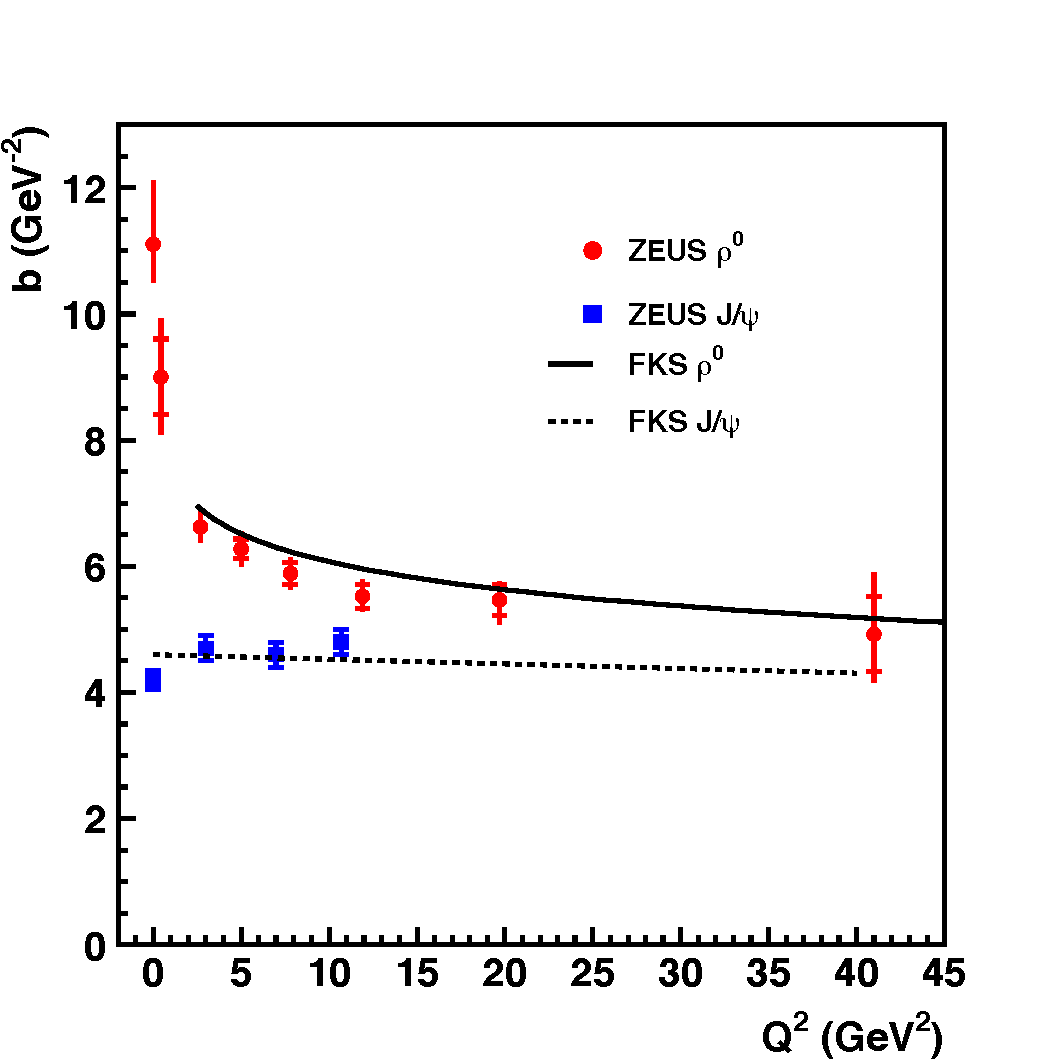
\includegraphics[width=0.6\textwidth]{chap2/hera.pdf}
    \caption{The results of a parameterization,
             $\frac{d\sigma}{dt}\propto e^{-bt}$, of the $\rho$ and $J/\psi$
             electroproduction cross sections measured at HERA.
             The curves are predictions of the $Q^2$ dependence of $b$
             from~\cite{Frankfurt_1998}.
            }
    \label{fig:hera}
\end{figure}


